\chapter{Brugervejledning}

\section{Forestillinger}

Når Bookie åbnes, vises fanen \textit{Forestillinger}, der indeholder listen af forestillinger samt reservationsskærmen som set på figur \ref{screenshot:bookie}. På denne figur ses ydermere følgende elementer: Placeringen af lærredet i biografsalen, legenden over sædestatus (ledig, valgt, reserveret, og købt), samt formularen til reservation af sæder. En biografsal er imidlertid endnu ikke synlig, da der ikke er valgt en forestilling.

\begin{figure}[h]
  \centering
  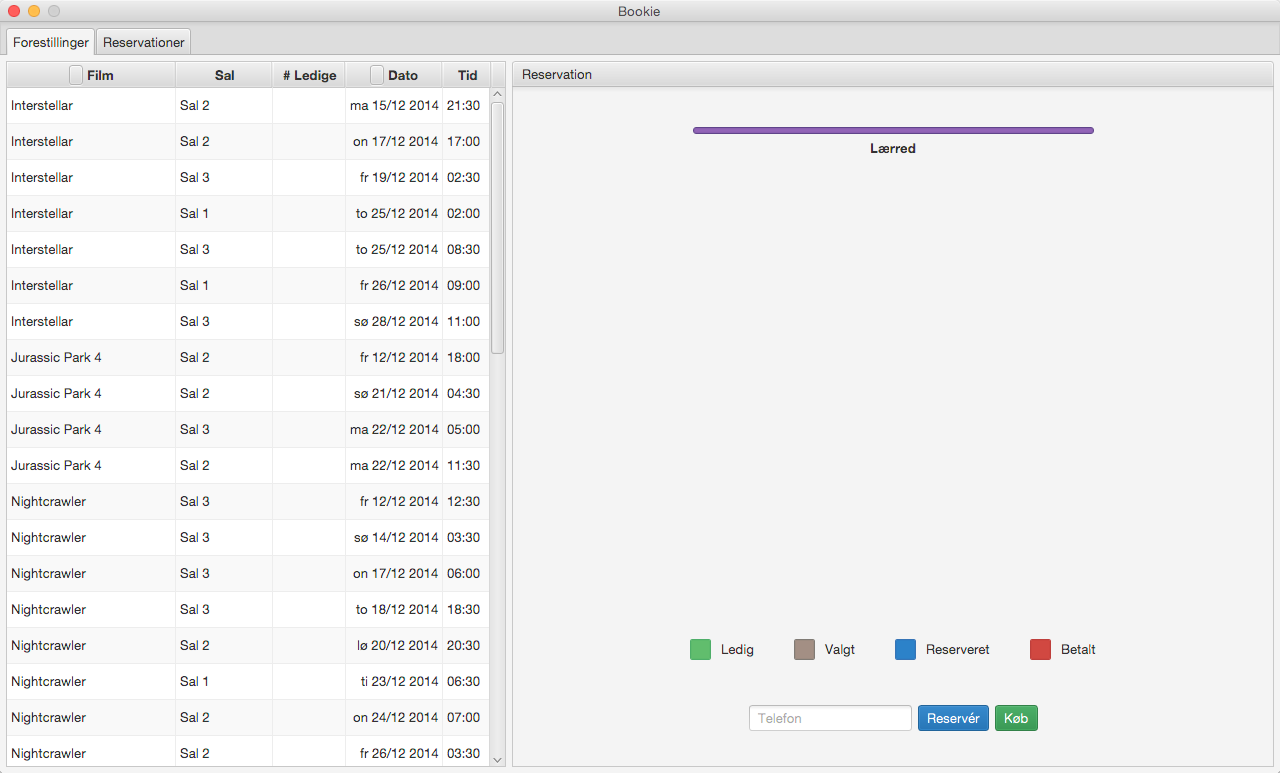
\includegraphics[width=\textwidth]{bookie.png}
  \caption{Bookies startside straks efter opstart}
  \label{screenshot:bookie}
\end{figure}

\subsection{Valg af forestilling}

Der er mulighed for at sortere listen af forestillinger efter film, sal, ledige sæder, dato, og tidspunkt. Det er derfor let at finde præcist den forestilling, som kunden måtte ønske.

%I tilfælde af, at listen med forestillinger bliver uoverskueligt lang, kan den filtreres på enten film eller dato således, at kun et ønsket udsnit af forestillinger er synlige på listen.

På figur \ref{screenshot:chosen-showtime}) er vist hvorledes en forestillingen vælges, hvorefter dennes biografsal bliver synlig på skærmen.

\begin{figure}[h]
  \centering
  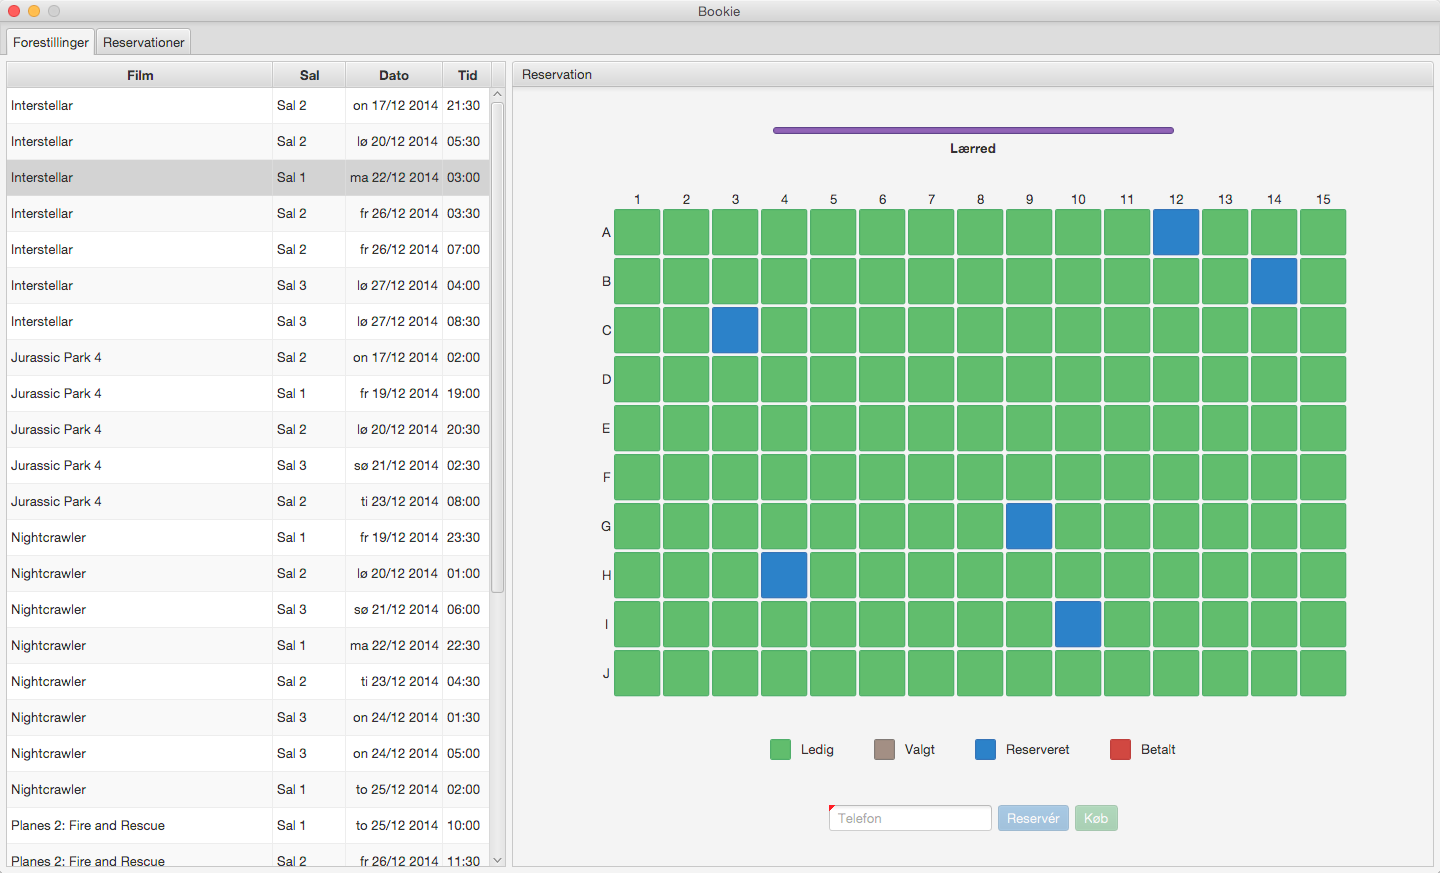
\includegraphics[width=\textwidth]{chosen-showtime.png}
  \caption{Udseende af biografsalen efter valg af forestilling}
  \label{screenshot:chosen-showtime}
\end{figure}

\subsection{Valg af sæder}

\begin{wrapfigure}[4]{r}{0.4\textwidth}
  \centering
  \vspace{-12pt}
  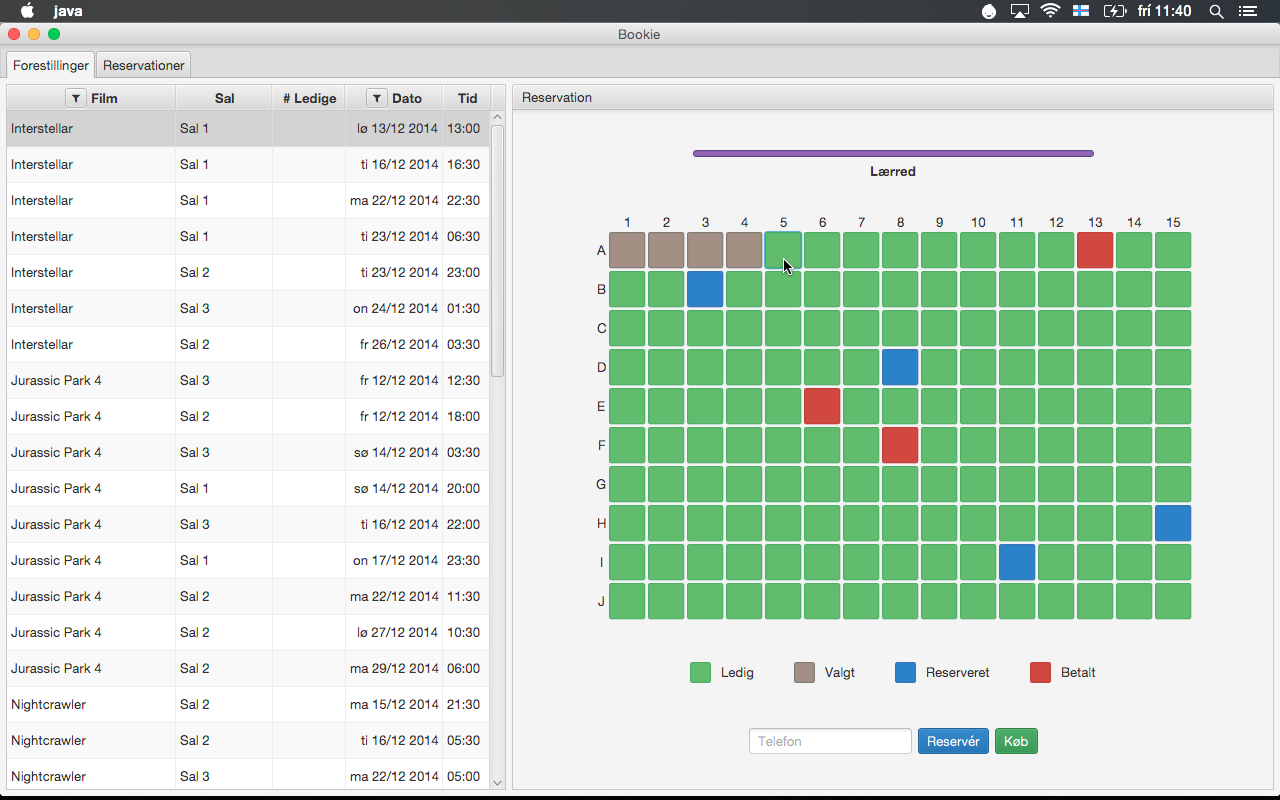
\includegraphics[width=0.35\textwidth]{chosen-seats.png}
  \caption{Eksempel på valg af sæder}
  \label{screenshot:chosen-seats}
\end{wrapfigure}

Sæderne er angivet i rækker og kolonner, hvor rækkerne har navne efter alfabetet og kolonnerne efter tal. Holdes musen hen over et af de ledige sæder (markerede med grøn) og trykkes der på det, vil sædet skifte farve til grå som indikation på, at det er valgt til reservation.

\subsection{Reservation af sæder}

\begin{wrapfigure}[4]{r}{0.4\textwidth}
  \centering
  \vspace{-12pt}
  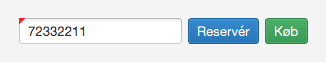
\includegraphics[width=0.35\textwidth]{phone-number.png}
  \caption{Et telefonnr. bliver indtastet}
  \label{screenshot:phone-number}
\end{wrapfigure}

Efter at de ønskede sæder er blevet valgt, er det muligt at indtaste et telefonnummer (se figur \ref{screenshot:phone-number}) for reservationen. Trykkes der derefter på \textit{Reservér}-knappen, ændres sædernes farve til blå som indikation på, at reservationen er gennemført.

%\begin{figure}[h]
%  \centering
%  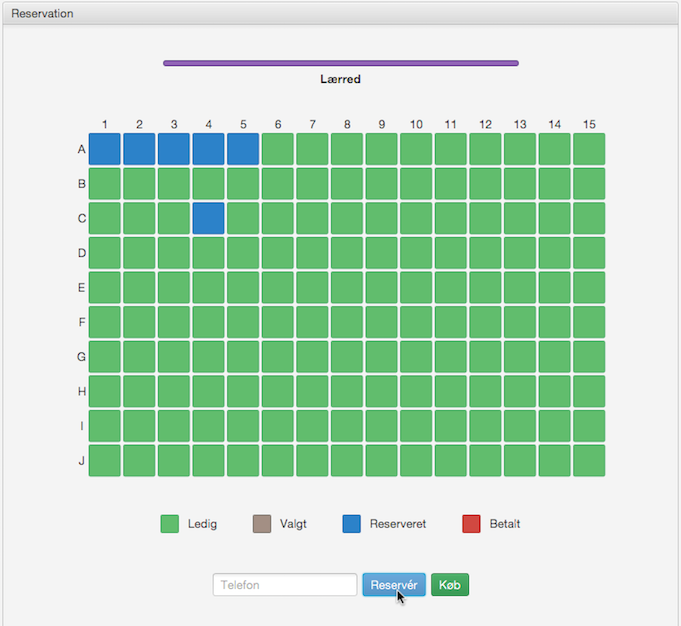
\includegraphics[width=0.4\textwidth]{booked-seats.png}
%  \caption{Reserverede sæder.}
%  \label{screenshot:booked-seats}
%\end{figure}

\section{Reservationer}

\begin{wrapfigure}[3]{r}{0.4\textwidth}
  \centering
  \vspace{-12pt}
  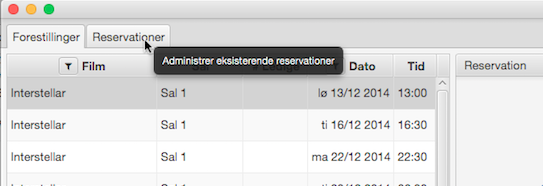
\includegraphics[width=0.35\textwidth]{go-to-reservations.png}
  \caption{Gå til alle reservationer.}
  \label{screenshot:go-to-reservations}
\end{wrapfigure}

Når en reservation er oprettet, kan denne findes under fanen \textit{Reservationer} (figur \ref{screenshot:go-to-reservations}). Alle eksisterende reservationer kan ligeledes findes under denne fane som set på figur \ref{screenshot:all-reservations}.

\begin{figure}[h]
  \centering
  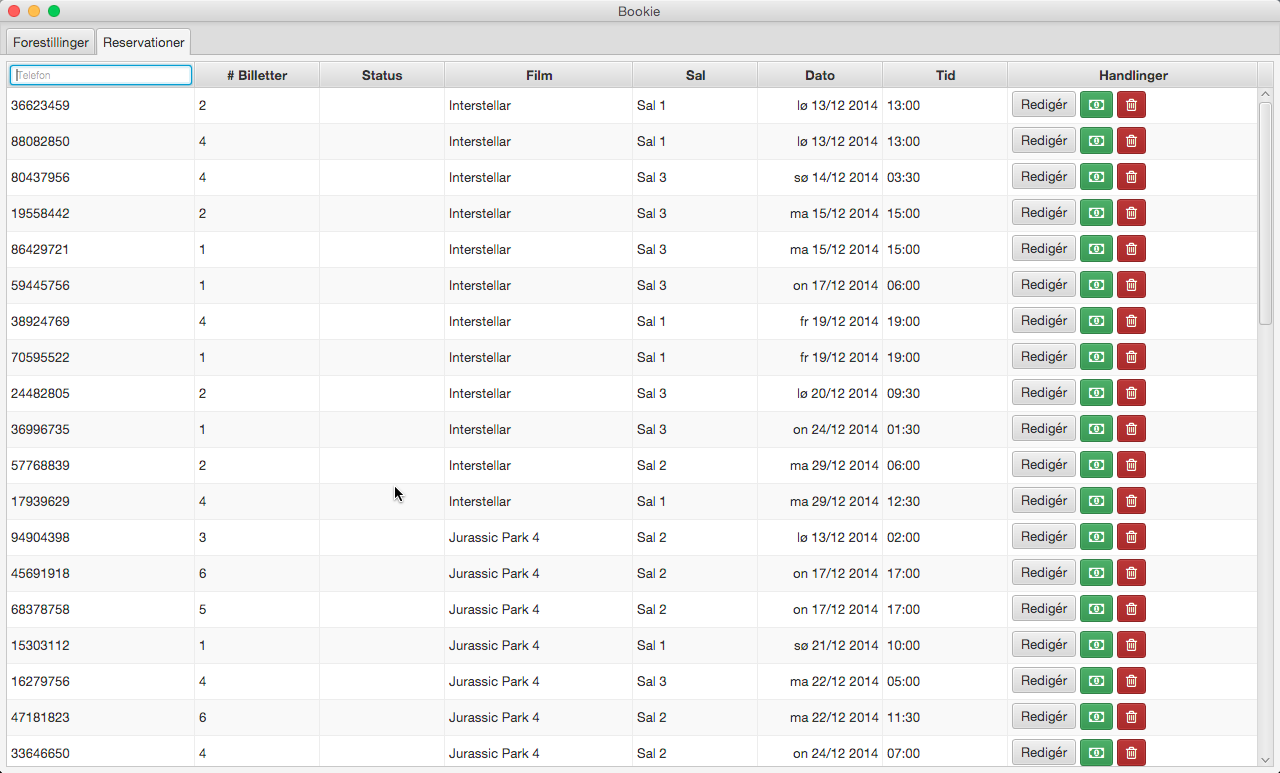
\includegraphics[width=\textwidth]{all-reservations.png}
  \caption{Alle reservationer bliver vist.}
  \label{screenshot:all-reservations}
\end{figure}

\subsection{Filtrering af telefonnumre}

\begin{wrapfigure}[3]{r}{0.4\textwidth}
  \centering
  \vspace{-12pt}
  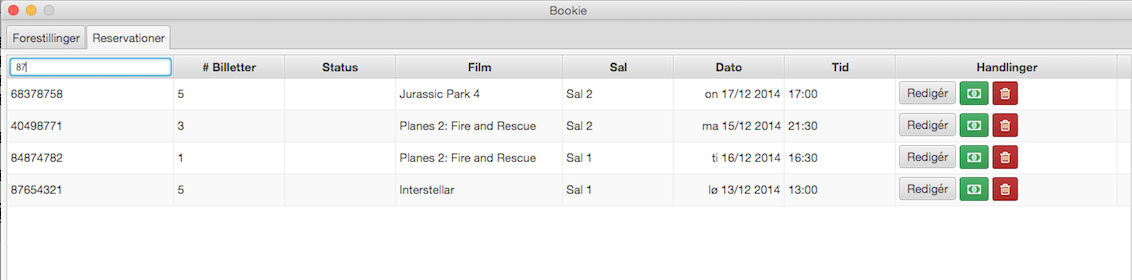
\includegraphics[width=0.35\textwidth]{filter3.png}
  \caption{Filtrering af telefonnumre}
  \label{screenshot:filter3}
\end{wrapfigure}

I øverste, venstre hjørne af reservationslisten findes et felt til filtrering af telefonnumrene (figur \ref{screenshot:filter3}). Der kan søges på enten fulde telefonnumre eller brydstykker af disse, hvilket gør det let af finde den/de ønskede reservationer.

\subsection{Redigering af reservationer}

\begin{wrapfigure}{r}{0.4\textwidth}
  \centering
  \vspace{-12pt}
  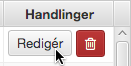
\includegraphics[width=0.35\textwidth]{edit-button.png}
  \caption{Mulighed for at redigere den enkelte reservation.}
  \label{screenshot:edit-button}
\end{wrapfigure}

Når den ønskede reservation er fundet, kan denne hurtigt redigeres ved at trykke på \textit{Redigér}-knappen fundet i højre side af skærmen (figur \ref{screenshot:edit-button}). \textit{Forestillinger}-fanen vil da blive vist, hvorefter der enten kan fjernes eller tilføjes flere sæder til den pågældende reservation (figur \ref{screenshot:edit1}).

%Hvis det skulle ske, at kunden vil ændre reservationen således, at han/hun vil se den valgte film på et andet tidspunkt, så vil ekspedienten slette hele reservationen og oprette en ny, da Bookie ikke er lavet til at flytte reservationerne fra tidspunkt til tidspunkt.

\subsection{Sletning af reservationer}

\begin{wrapfigure}{r}{0.4\textwidth}
  \centering
  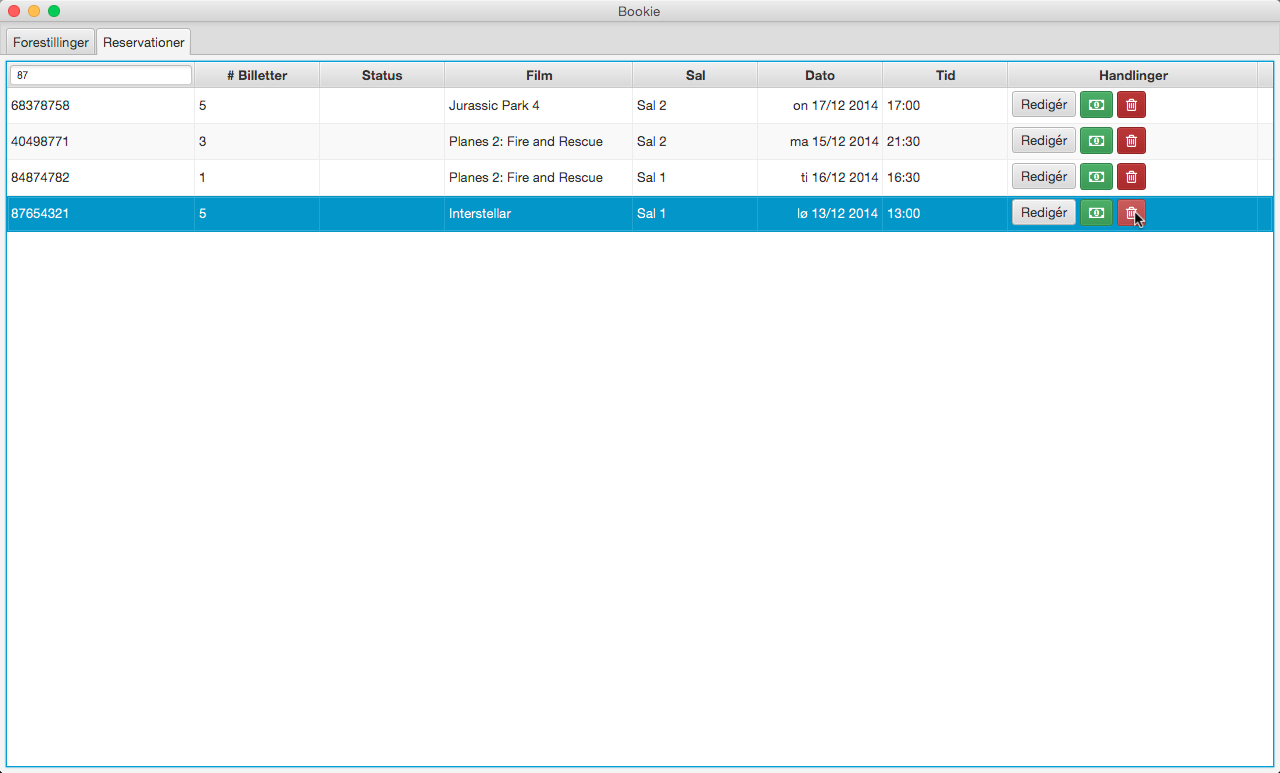
\includegraphics[width=0.35\textwidth]{delete-button.png}
  \caption{Mulighed for at slette den enkelte reservation.}
  \label{screenshot:delete-button}
\end{wrapfigure}

At slette er reservation er lige så smertefrit som at arbejde i resten af Bookie. Bliver der trykket på den røde knap med skraldespand-ikonet ved siden af \textit{redigér} knappen (som ses på \ref{screenshot:delete-button}, så kommer et pop-up (figur \ref{screenshot:delete-reservation}, hvor man kan vælge mellem \textit{cancel} eller \textit{ok}. Vælger ekspedienten \textit{cancel}, sker der ikke noget andet end, at pop-up'et forsvinder og \textit{Reservationer} forbliver som før. Vælger ekspedienten \textit{ok}, forsvinder den valgte reservation fra listen (figur \ref{screenshot:after-delete}).

\begin{figure} [h]
  \centering
  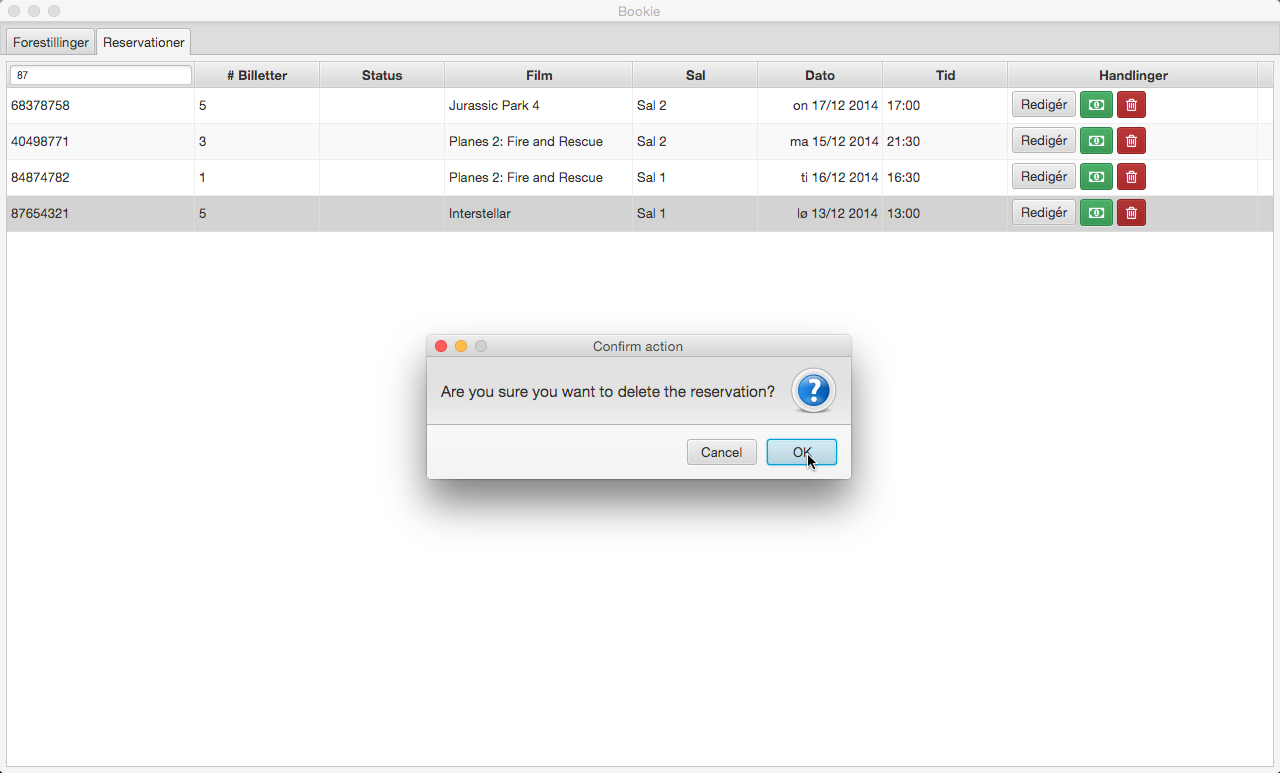
\includegraphics[width=0.4\textwidth]{delete-reservation.png}
  \caption{Sletning af reservation.}
  \label{screenshot:delete-reservation}
\end{figure}

\begin{figure}[h]
  \centering
  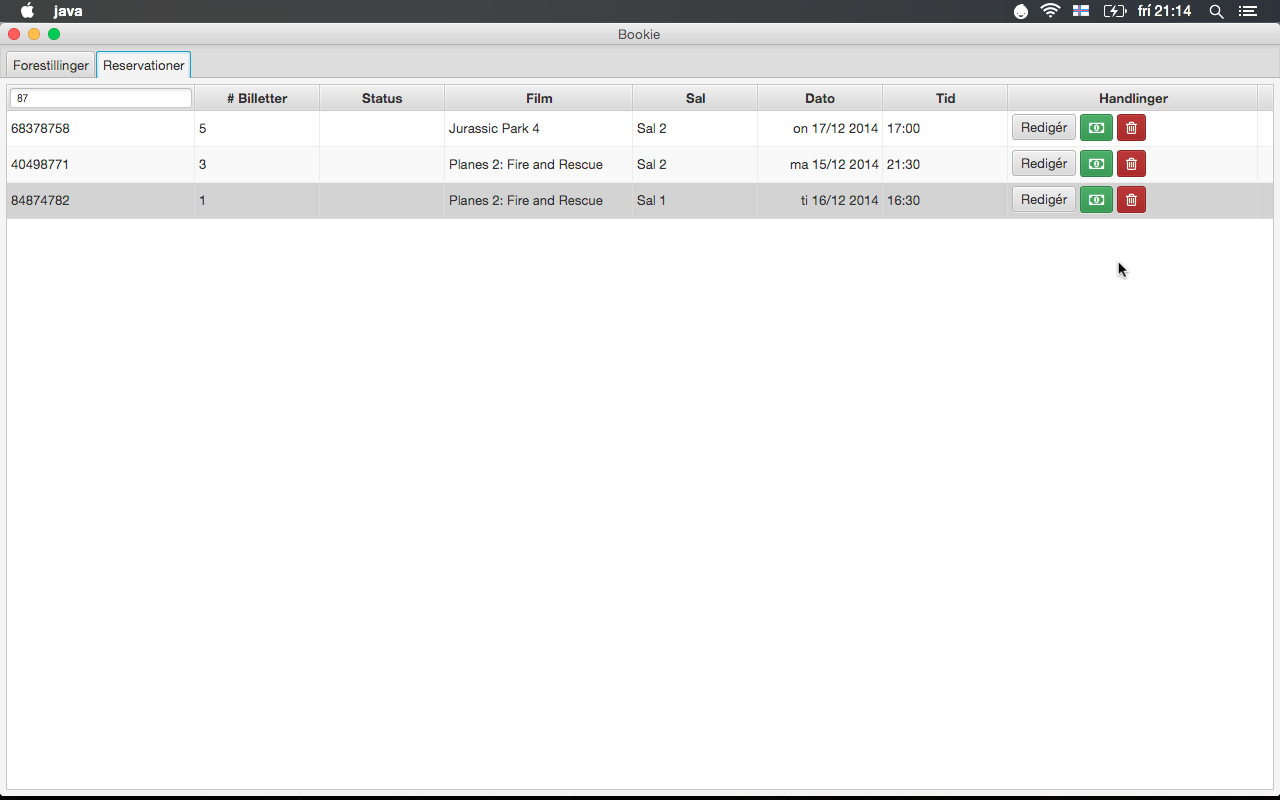
\includegraphics[width=0.4\textwidth]{after-delete.png}
  \caption{Efter at en reservation er slettet.}
  \label{screenshot:after-delete}
\end{figure}

Det viser sig, at det er meget nemt for ekspedienten at finde rundt i Bookie. Hvilket er meget godt, da der kan være meget pres, f.eks. til premieren til \textit{The Hobbit - The Battle of the Five Armies} her i december måned. Selv om der kun er én ekspedient der kan bruge Bookie ad gangen, så må man kunne holde hovedet koldt, når der skal serviceres en billetluge og en telefon på samme tid.